\chapter{Semantička analiza}

\section{Uvod}

Cilj semantičke analize je provjeriti i odrediti značenje pojedinih dijelova programa npr. provjeriti
je li varijabla koja se koristi deklarirana, odrediti tip podataka koji pripada nekom čvoru (npr. tipa \texttt{expr}
koji predstavlja aritmetičko-logički izraz).

Često se koristi sintaksnom vođena semantička analiza na način da se završni i nezavršni znakovi gramatike
prošire s atributima koji se izračunavaju prilikom parsiranja. CUP podržava takav način rada, no
mi ga nismo koristili. Naknadno, kad već dobijemo sintaksno stablo, obilazimo čvorove.

U našem jezičnom procesoru provjeravamo dvije osnovne stvari prilikom semantičke analize. Prva je da pazimo
na djelokruge varijabli i jesu li dostupne prilikom korištenja (jesu li uopće deklarirane). A druga je
da provjeravamo tipove podataka izraza. Informacije koje na taj način prikupimo prilikom semantičke
analize su nam iznimno bitne za generiranje ciljnog programa.


\section{Implementacija}
Semantički analizator je implementiran u razredu \texttt{SemanticAnalyzer}. Pozivom metode \texttt{analyze()}
pokreće se (ili nastavlja) analiza.

Prilikom analize obilazimo sintaksno stablo. Za to koristimo stog na koji stavljamo čvorove stabla.
U nekom koraku obilaska sa stoga skinemo jedan čvor, svu njegovu djecu stavimo na stog ali obrnutim redoslijedom i 
obradimo skinuti čvor (često jednostavno nastavimo s obilaskom po stablu). To ponavljamo dok na stogu ima čvorova za obraditi. 
Na početku se na vrhu stoga nalazi vrh sintaksnog stabla.
Za određene tipove čvorova su definirane akcije koje se izvrše kada posjetimo te čvorove. 

Ukoliko posjetimo čvor tipa \texttt{expr} i za njega nije određen tip podataka onda rekurzivno 
odredimo tip. Na taj način se izvodi prvi dio semantičke analize. Drugi dio je malo kompliciraniji.

Izvorni jezik ima statički djelokrug bez ugnježđenja funkcija. 

Uz stog koji koristimo za obilazak, koristimo i stog na kojem čuvamo djelokruge. Djelokrug
je predstavljen razredom \texttt{Scope} i sastoji se u suštini od par hash-mapi koje čuvaju
popis varijabli koje su deklarirane u tom djelokrugu, njihov tip i redni broj deklaracije (bitno za generiranje ciljnog programa).
Na vrhu tog stoga je uvijek trenutni aktivni djelokrug i sve deklaracije na koje naiđemo se odnose na njega.
Ukoliko se neka varijabla koristi u nekom izrazu onda provjerimo sve djelokruge (počevši od vrha stoga prema dnu)
sadrže li tu varijablu. Na početku je na vrhu stoga globalni djelokrug.

Ukoliko se dogodi da neka varijabla nije deklarirana, a pokuša se koristiti onda se prijavljuje greška. Semantička
analiza se nastavlja, no nakon nje, ukoliko postoje greške, ne pokreće se generiranje izlaznog koda.

Nije implementirana provjera broja argumenata koje funkcija prima.

\section{Primjer izvođenja i određivanja djelokruga}
Pogledajmo primjer određivanja djelokruga varijabli.

\lstinputlisting[language=C]{primjer-semanticka1.c}

\begin{figure}[H]
  \centering
    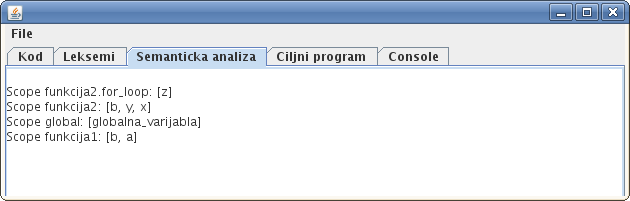
\includegraphics[width=13cm]{primjer-semanticka1}
  \caption{Primjer izvođenja semantičke analize}
\end{figure}

\pagebreak

Pogledajmo i jedan primjer gdje se koristi varijabla koja nije deklarirana (varijabla \texttt{z}).
\lstinputlisting[language=C]{primjer-semanticka2.c}

\begin{figure}[H]
  \centering
    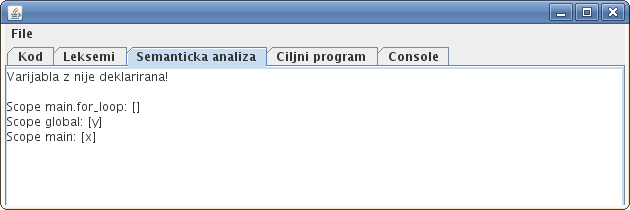
\includegraphics[width=13cm]{primjer-semanticka2}
  \caption{Primjer izvođenja semantičke analize s greškom u programu}
\label{komponente}
\end{figure}

